
%% for title page




%% bare_jrnl.tex
%% V1.3
%% 2007/01/11
%% by Michael Shell
%% see http://www.michaelshell.org/
%% for current contact information.
%%
%% This is a skeleton file demonstrating the use of IEEEtran.cls
%% (requires IEEEtran.cls version 1.7 or later) with an IEEE journal paper.
%%
%% Support sites:
%% http://www.michaelshell.org/tex/ieeetran/
%% http://www.ctan.org/tex-archive/macros/latex/contrib/IEEEtran/
%% and
%% http://www.ieee.org/



% *** Authors should verify (and, if needed, correct) their LaTeX system  ***
% *** with the testflow diagnostic prior to trusting their LaTeX platform ***
% *** with production work. IEEE's font choices can trigger bugs that do  ***
% *** not appear when using other class files.                            ***
% The testflow support page is at:
% http://www.michaelshell.org/tex/testflow/


%%*************************************************************************
%% Legal Notice:
%% This code is offered as-is without any warranty either expressed or
%% implied; without even the implied warranty of MERCHANTABILITY or
%% FITNESS FOR A PARTICULAR PURPOSE! 
%% User assumes all risk.
%% In no event shall IEEE or any contributor to this code be liable for
%% any damages or losses, including, but not limited to, incidental,
%% consequential, or any other damages, resulting from the use or misuse
%% of any information contained here.
%%
%% All comments are the opinions of their respective authors and are not
%% necessarily endorsed by the IEEE.
%%
%% This work is distributed under the LaTeX Project Public License (LPPL)
%% ( http://www.latex-project.org/ ) version 1.3, and may be freely used,
%% distributed and modified. A copy of the LPPL, version 1.3, is included
%% in the base LaTeX documentation of all distributions of LaTeX released
%% 2003/12/01 or later.
%% Retain all contribution notices and credits.
%% ** Modified files should be clearly indicated as such, including  **
%% ** renaming them and changing author support contact information. **
%%
%% File list of work: IEEEtran.cls, IEEEtran_HOWTO.pdf, bare_adv.tex,
%%                    bare_conf.tex, bare_jrnl.tex, bare_jrnl_compsoc.tex
%%*************************************************************************

% Note that the a4paper option is mainly intended so that authors in
% countries using A4 can easily print to A4 and see how their papers will
% look in print - the typesetting of the document will not typically be
% affected with changes in paper size (but the bottom and side margins will).
% Use the testflow package mentioned above to verify correct handling of
% both paper sizes by the user's LaTeX system.
%
% Also note that the "draftcls" or "draftclsnofoot", not "draft", option
% should be used if it is desired that the figures are to be displayed in
% draft mode.
%
\documentclass[journal]{IEEEtran}

\usepackage{amsmath}


% for title page
\usepackage[utf8]{inputenc} % Required for inputting international characters
\usepackage[T1]{fontenc} % Output font encoding for international characters
\usepackage{mathpazo} % Palatino font


\usepackage{blindtext}
\usepackage{graphicx}

% to patch the bibliography with section, so no page break
\usepackage{etoolbox}
\patchcmd{\thebibliography}{\chapter*}{\section*}{}{}

\usepackage{multirow}% http://ctan.org/pkg/multirow
\usepackage{hhline}% http://ctan.org/pkg/hhline
\usepackage{tabularx,booktabs}
\newcolumntype{C}{>{\centering\arraybackslash}X} % centered version of "X" type
\setlength{\extrarowheight}{1pt}

\usepackage{rotating}

\usepackage{lipsum}

% Some very useful LaTeX packages include:
% (uncomment the ones you want to load)


% *** MISC UTILITY PACKAGES ***
%
%\usepackage{ifpdf}
% Heiko Oberdiek's ifpdf.sty is very useful if you need conditional
% compilation based on whether the output is pdf or dvi.
% usage:
% \ifpdf
%   % pdf code
% \else
%   % dvi code
% \fi
% The latest version of ifpdf.sty can be obtained from:
% http://www.ctan.org/tex-archive/macros/latex/contrib/oberdiek/
% Also, note that IEEEtran.cls V1.7 and later provides a builtin
% \ifCLASSINFOpdf conditional that works the same way.
% When switching from latex to pdflatex and vice-versa, the compiler may
% have to be run twice to clear warning/error messages.






% *** CITATION PACKAGES ***
%
%\usepackage{cite}
\usepackage{url}


% cite.sty was written by Donald Arseneau
% V1.6 and later of IEEEtran pre-defines the format of the cite.sty package
% \cite{} output to follow that of IEEE. Loading the cite package will
% result in citation numbers being automatically sorted and properly
% "compressed/ranged". e.g., [1], [9], [2], [7], [5], [6] without using
% cite.sty will become [1], [2], [5]--[7], [9] using cite.sty. cite.sty's
% \cite will automatically add leading space, if needed. Use cite.sty's
% noadjust option (cite.sty V3.8 and later) if you want to turn this off.
% cite.sty is already installed on most LaTeX systems. Be sure and use
% version 4.0 (2003-05-27) and later if using hyperref.sty. cite.sty does
% not currently provide for hyperlinked citations.
% The latest version can be obtained at:
% http://www.ctan.org/tex-archive/macros/latex/contrib/cite/
% The documentation is contained in the cite.sty file itself.






% *** GRAPHICS RELATED PACKAGES ***
%
\ifCLASSINFOpdf
  % \usepackage[pdftex]{graphicx}
  % declare the path(s) where your graphic files are
  % \graphicspath{{../pdf/}{../jpeg/}}
  % and their extensions so you won't have to specify these with
  % every instance of \includegraphics
  % \DeclareGraphicsExtensions{.pdf,.jpeg,.png}
\else
  % or other class option (dvipsone, dvipdf, if not using dvips). graphicx
  % will default to the driver specified in the system graphics.cfg if no
  % driver is specified.
  % \usepackage[dvips]{graphicx}
  % declare the path(s) where your graphic files are
  % \graphicspath{{../eps/}}
  % and their extensions so you won't have to specify these with
  % every instance of \includegraphics
  % \DeclareGraphicsExtensions{.eps}
\fi
% graphicx was written by David Carlisle and Sebastian Rahtz. It is
% required if you want graphics, photos, etc. graphicx.sty is already
% installed on most LaTeX systems. The latest version and documentation can
% be obtained at: 
% http://www.ctan.org/tex-archive/macros/latex/required/graphics/
% Another good source of documentation is "Using Imported Graphics in
% LaTeX2e" by Keith Reckdahl which can be found as epslatex.ps or
% epslatex.pdf at: http://www.ctan.org/tex-archive/info/
%
% latex, and pdflatex in dvi mode, support graphics in encapsulated
% postscript (.eps) format. pdflatex in pdf mode supports graphics
% in .pdf, .jpeg, .png and .mps (metapost) formats. Users should ensure
% that all non-photo figures use a vector format (.eps, .pdf, .mps) and
% not a bitmapped formats (.jpeg, .png). IEEE frowns on bitmapped formats
% which can result in "jaggedy"/blurry rendering of lines and letters as
% well as large increases in file sizes.
%
% You can find documentation about the pdfTeX application at:
% http://www.tug.org/applications/pdftex





% *** MATH PACKAGES ***
%
%\usepackage[cmex10]{amsmath}
% A popular package from the American Mathematical Society that provides
% many useful and powerful commands for dealing with mathematics. If using
% it, be sure to load this package with the cmex10 option to ensure that
% only type 1 fonts will utilized at all point sizes. Without this option,
% it is possible that some math symbols, particularly those within
% footnotes, will be rendered in bitmap form which will result in a
% document that can not be IEEE Xplore compliant!
%
% Also, note that the amsmath package sets \interdisplaylinepenalty to 10000
% thus preventing page breaks from occurring within multiline equations. Use:
%\interdisplaylinepenalty=2500
% after loading amsmath to restore such page breaks as IEEEtran.cls normally
% does. amsmath.sty is already installed on most LaTeX systems. The latest
% version and documentation can be obtained at:
% http://www.ctan.org/tex-archive/macros/latex/required/amslatex/math/





% *** SPECIALIZED LIST PACKAGES ***
%
%\usepackage{algorithmic}
% algorithmic.sty was written by Peter Williams and Rogerio Brito.
% This package provides an algorithmic environment fo describing algorithms.
% You can use the algorithmic environment in-text or within a figure
% environment to provide for a floating algorithm. Do NOT use the algorithm
% floating environment provided by algorithm.sty (by the same authors) or
% algorithm2e.sty (by Christophe Fiorio) as IEEE does not use dedicated
% algorithm float types and packages that provide these will not provide
% correct IEEE style captions. The latest version and documentation of
% algorithmic.sty can be obtained at:
% http://www.ctan.org/tex-archive/macros/latex/contrib/algorithms/
% There is also a support site at:
% http://algorithms.berlios.de/index.html
% Also of interest may be the (relatively newer and more customizable)
% algorithmicx.sty package by Szasz Janos:
% http://www.ctan.org/tex-archive/macros/latex/contrib/algorithmicx/




% *** ALIGNMENT PACKAGES ***
%
%\usepackage{array}
% Frank Mittelbach's and David Carlisle's array.sty patches and improves
% the standard LaTeX2e array and tabular environments to provide better
% appearance and additional user controls. As the default LaTeX2e table
% generation code is lacking to the point of almost being broken with
% respect to the quality of the end results, all users are strongly
% advised to use an enhanced (at the very least that provided by array.sty)
% set of table tools. array.sty is already installed on most systems. The
% latest version and documentation can be obtained at:
% http://www.ctan.org/tex-archive/macros/latex/required/tools/


%\usepackage{mdwmath}
%\usepackage{mdwtab}
% Also highly recommended is Mark Wooding's extremely powerful MDW tools,
% especially mdwmath.sty and mdwtab.sty which are used to format equations
% and tables, respectively. The MDWtools set is already installed on most
% LaTeX systems. The lastest version and documentation is available at:
% http://www.ctan.org/tex-archive/macros/latex/contrib/mdwtools/


% IEEEtran contains the IEEEeqnarray family of commands that can be used to
% generate multiline equations as well as matrices, tables, etc., of high
% quality.


%\usepackage{eqparbox}
% Also of notable interest is Scott Pakin's eqparbox package for creating
% (automatically sized) equal width boxes - aka "natural width parboxes".
% Available at:
% http://www.ctan.org/tex-archive/macros/latex/contrib/eqparbox/





% *** SUBFIGURE PACKAGES ***
%\usepackage[tight,footnotesize]{subfigure}
% subfigure.sty was written by Steven Douglas Cochran. This package makes it
% easy to put subfigures in your figures. e.g., "Figure 1a and 1b". For IEEE
% work, it is a good idea to load it with the tight package option to reduce
% the amount of white space around the subfigures. subfigure.sty is already
% installed on most LaTeX systems. The latest version and documentation can
% be obtained at:
% http://www.ctan.org/tex-archive/obsolete/macros/latex/contrib/subfigure/
% subfigure.sty has been superceeded by subfig.sty.



%\usepackage[caption=false]{caption}
%\usepackage[font=footnotesize]{subfig}
% subfig.sty, also written by Steven Douglas Cochran, is the modern
% replacement for subfigure.sty. However, subfig.sty requires and
% automatically loads Axel Sommerfeldt's caption.sty which will override
% IEEEtran.cls handling of captions and this will result in nonIEEE style
% figure/table captions. To prevent this problem, be sure and preload
% caption.sty with its "caption=false" package option. This is will preserve
% IEEEtran.cls handing of captions. Version 1.3 (2005/06/28) and later 
% (recommended due to many improvements over 1.2) of subfig.sty supports
% the caption=false option directly:
%\usepackage[caption=false,font=footnotesize]{subfig}
%
% The latest version and documentation can be obtained at:
% http://www.ctan.org/tex-archive/macros/latex/contrib/subfig/
% The latest version and documentation of caption.sty can be obtained at:
% http://www.ctan.org/tex-archive/macros/latex/contrib/caption/




% *** FLOAT PACKAGES ***
%
%\usepackage{fixltx2e}
% fixltx2e, the successor to the earlier fix2col.sty, was written by
% Frank Mittelbach and David Carlisle. This package corrects a few problems
% in the LaTeX2e kernel, the most notable of which is that in current
% LaTeX2e releases, the ordering of single and double column floats is not
% guaranteed to be preserved. Thus, an unpatched LaTeX2e can allow a
% single column figure to be placed prior to an earlier double column
% figure. The latest version and documentation can be found at:
% http://www.ctan.org/tex-archive/macros/latex/base/



%\usepackage{stfloats}
% stfloats.sty was written by Sigitas Tolusis. This package gives LaTeX2e
% the ability to do double column floats at the bottom of the page as well
% as the top. (e.g., "\begin{figure*}[!b]" is not normally possible in
% LaTeX2e). It also provides a command:
%\fnbelowfloat
% to enable the placement of footnotes below bottom floats (the standard
% LaTeX2e kernel puts them above bottom floats). This is an invasive package
% which rewrites many portions of the LaTeX2e float routines. It may not work
% with other packages that modify the LaTeX2e float routines. The latest
% version and documentation can be obtained at:
% http://www.ctan.org/tex-archive/macros/latex/contrib/sttools/
% Documentation is contained in the stfloats.sty comments as well as in the
% presfull.pdf file. Do not use the stfloats baselinefloat ability as IEEE
% does not allow \baselineskip to stretch. Authors submitting work to the
% IEEE should note that IEEE rarely uses double column equations and
% that authors should try to avoid such use. Do not be tempted to use the
% cuted.sty or midfloat.sty packages (also by Sigitas Tolusis) as IEEE does
% not format its papers in such ways.


%\ifCLASSOPTIONcaptionsoff
%  \usepackage[nomarkers]{endfloat}
% \let\MYoriglatexcaption\caption
% \renewcommand{\caption}[2][\relax]{\MYoriglatexcaption[#2]{#2}}
%\fi
% endfloat.sty was written by James Darrell McCauley and Jeff Goldberg.
% This package may be useful when used in conjunction with IEEEtran.cls'
% captionsoff option. Some IEEE journals/societies require that submissions
% have lists of figures/tables at the end of the paper and that
% figures/tables without any captions are placed on a page by themselves at
% the end of the document. If needed, the draftcls IEEEtran class option or
% \CLASSINPUTbaselinestretch interface can be used to increase the line
% spacing as well. Be sure and use the nomarkers option of endfloat to
% prevent endfloat from "marking" where the figures would have been placed
% in the text. The two hack lines of code above are a slight modification of
% that suggested by in the endfloat docs (section 8.3.1) to ensure that
% the full captions always appear in the list of figures/tables - even if
% the user used the short optional argument of \caption[]{}.
% IEEE papers do not typically make use of \caption[]'s optional argument,
% so this should not be an issue. A similar trick can be used to disable
% captions of packages such as subfig.sty that lack options to turn off
% the subcaptions:
% For subfig.sty:
% \let\MYorigsubfloat\subfloat
% \renewcommand{\subfloat}[2][\relax]{\MYorigsubfloat[]{#2}}
% For subfigure.sty:
% \let\MYorigsubfigure\subfigure
% \renewcommand{\subfigure}[2][\relax]{\MYorigsubfigure[]{#2}}
% However, the above trick will not work if both optional arguments of
% the \subfloat/subfig command are used. Furthermore, there needs to be a
% description of each subfigure *somewhere* and endfloat does not add
% subfigure captions to its list of figures. Thus, the best approach is to
% avoid the use of subfigure captions (many IEEE journals avoid them anyway)
% and instead reference/explain all the subfigures within the main caption.
% The latest version of endfloat.sty and its documentation can obtained at:
% http://www.ctan.org/tex-archive/macros/latex/contrib/endfloat/
%
% The IEEEtran \ifCLASSOPTIONcaptionsoff conditional can also be used
% later in the document, say, to conditionally put the References on a 
% page by themselves.





% *** PDF, URL AND HYPERLINK PACKAGES ***
%
%\usepackage{url}
% url.sty was written by Donald Arseneau. It provides better support for
% handling and breaking URLs. url.sty is already installed on most LaTeX
% systems. The latest version can be obtained at:
% http://www.ctan.org/tex-archive/macros/latex/contrib/misc/
% Read the url.sty source comments for usage information. Basically,
% \url{my_url_here}.





% *** Do not adjust lengths that control margins, column widths, etc. ***
% *** Do not use packages that alter fonts (such as pslatex).         ***
% There should be no need to do such things with IEEEtran.cls V1.6 and later.
% (Unless specifically asked to do so by the journal or conference you plan
% to submit to, of course. )


% correct bad hyphenation here
\hyphenation{op-tical net-works semi-conduc-tor}



%  \patchcmd{\abstract}{\titlepage}{\titlepage% Insert ToC-writing after starting a titlepage
%  \addcontentsline{toc}{section}{Abstract}}{}{}
  
\begin{document}

%%%%%%%%%%%%%%%%%%%%%%%%%%%%%%%%%%%%%%%%%
% Academic Title Page
% LaTeX Template
% Version 2.0 (17/7/17)
%
% This template was downloaded from:
% http://www.LaTeXTemplates.com
%
% Original author:
% WikiBooks (LaTeX - Title Creation) with modifications by:
% Vel (vel@latextemplates.com)
%
% License:
% CC BY-NC-SA 3.0 (http://creativecommons.org/licenses/by-nc-sa/3.0/)
% 
% Instructions for using this template:
% This title page is capable of being compiled as is. This is not useful for 
% including it in another document. To do this, you have two options: 
%
% 1) Copy/paste everything between \begin{document} and \end{document} 
% starting at \begin{titlepage} and paste this into another LaTeX file where you 
% want your title page.
% OR
% 2) Remove everything outside the \begin{titlepage} and \end{titlepage}, rename
% this file and move it to the same directory as the LaTeX file you wish to add it to. 
% Then add \input{./<new filename>.tex} to your LaTeX file where you want your
% title page.
%
%%%%%%%%%%%%%%%%%%%%%%%%%%%%%%%%%%%%%%%%%

%----------------------------------------------------------------------------------------
%	PACKAGES AND OTHER DOCUMENT CONFIGURATIONS
%----------------------------------------------------------------------------------------


%----------------------------------------------------------------------------------------
%	TITLE PAGE
%----------------------------------------------------------------------------------------

\begin{titlepage} % Suppresses displaying the page number on the title page and the subsequent page counts as page 1
	\newcommand{\HRule}{\rule{\linewidth}{0.5mm}} % Defines a new command for horizontal lines, change thickness here
	
	\center % Centre everything on the page
	
	%------------------------------------------------
	%	Headings
	%------------------------------------------------
	
	\textsc{\LARGE Santa Clara University}\\[1.5cm] % Main heading such as the name of your university/college
	
	\textsc{\Large COEN 281 Pattern Recognition and Data Mining}\\[0.5cm] % Major heading such as course name
	
	\textsc{\large Term Project}\\[0.5cm] % Minor heading such as course title
	
	%------------------------------------------------
	%	Title
	%------------------------------------------------
	
	\HRule\\[0.4cm]
	
	{\huge\bfseries Finding Topics That Have Limited Supports on Stack Overflow}\\[0.4cm] % Title of your document
	
	\HRule\\[1.5cm]
	
	%------------------------------------------------
	%	Author(s)
	%------------------------------------------------
	
	\begin{minipage}{0.4\textwidth}
		\begin{flushleft}
			\large
			\textit{Author}\\
			Ting-yu \textsc{Yeh}\\ % Your name
			Nicholas \textsc{Fong}\\ % Your name
			Christian \textsc{Ayscue}\\ % Your name
			Bing \textsc{Tang}\\ % Your name			
		\end{flushleft}		
	\end{minipage}
	~
	\begin{minipage}{0.4\textwidth}
		\begin{flushright}
			\large
			\textit{Supervisor}\\
			Dr. Ming-Hwa \textsc{Wang} % Supervisor's name
		\end{flushright}
	\end{minipage}
	
	% If you don't want a supervisor, uncomment the two lines below and comment the code above
	%{\large\textit{Author}}\\
	%John \textsc{Smith} % Your name
	
	%------------------------------------------------
	%	Date
	%------------------------------------------------
	
	\vfill\vfill\vfill % Position the date 3/4 down the remaining page
	
	{\large\today} % Date, change the \today to a set date if you want to be precise
	
	%------------------------------------------------
	%	Logo
	%------------------------------------------------
	
	%\vfill\vfill
	%\includegraphics[width=0.2\textwidth]{placeholder.jpg}\\[1cm] % Include a department/university logo - this will require the graphicx package
	 
	%----------------------------------------------------------------------------------------
	
	\vfill % Push the date up 1/4 of the remaining page
	
\end{titlepage}

%----------------------------------------------------------------------------------------



\onecolumn
\tableofcontents
\listoffigures
\listoftables
\input{1_section1}
\newpage 
%
%\input{1_section1}
%\newpage

\twocolumn   
%
% paper title
% can use linebreaks \\ within to get better formatting as desired
\title{Finding Topics That Have Limited Supports on Stack Overflow}
%
%
% author names and IEEE memberships
% note positions of commas and nonbreaking spaces ( ~ ) LaTeX will not break
% a structure at a ~ so this keeps an author's name from being broken across
% two lines.
% use \thanks{} to gain access to the first footnote area
% a separate \thanks must be used for each paragraph as LaTeX2e's \thanks
% was not built to handle multiple paragraphs
%

\author{Ting-yu~Yeh,
        Nicholas Fong,
		Christian Ayscue,
        and~Bing Tang
\thanks{T. Yeh, N. Fong, C. Ayscue, and B. Tang are with the Department
of Computer Engineering, Santa Clara University, Santa Clara,
CA, 95053 USA}% <-this % stops a space
%\thanks{J. Doe and J. Doe are with Anonymous University.}% <-this % stops a space
%\thanks{Manuscript received April 19, 2005; revised January 11, 2007.}
}
% note the % following the last \IEEEmembership and also \thanks - 
% these prevent an unwanted space from occurring between the last author name
% and the end of the author line. i.e., if you had this:
% 
% \author{....lastname \thanks{...} \thanks{...} }
%                     ^------------^------------^----Do not want these spaces!
%
% a space would be appended to the last name and could cause every name on that
% line to be shifted left slightly. This is one of those "LaTeX things". For
% instance, "\textbf{A} \textbf{B}" will typeset as "A B" not "AB". To get
% "AB" then you have to do: "\textbf{A}\textbf{B}"
% \thanks is no different in this regard, so shield the last } of each \thanks
% that ends a line with a % and do not let a space in before the next \thanks.
% Spaces after \IEEEmembership other than the last one are OK (and needed) as
% you are supposed to have spaces between the names. For what it is worth,
% this is a minor point as most people would not even notice if the said evil
% space somehow managed to creep in.



% The paper headers
\markboth{Term Project of COEN 281, Pattern Recognition and Data Mining, Fall~2017}%
{Shell \MakeLowercase{\textit{et al.}}: Bare Demo of IEEEtran.cls for Journals}
% The only time the second header will appear is for the odd numbered pages
% after the title page when using the twoside option.
% 
% *** Note that you probably will NOT want to include the author's ***
% *** name in the headers of peer review papers.                   ***
% You can use \ifCLASSOPTIONpeerreview for conditional compilation here if
% you desire.




% If you want to put a publisher's ID mark on the page you can do it like
% this:
%\IEEEpubid{0000--0000/00\$00.00~\copyright~2007 IEEE}
% Remember, if you use this you must call \IEEEpubidadjcol in the second
% column for its text to clear the IEEEpubid mark.



% use for special paper notices
%\IEEEspecialpapernotice{(Invited Paper)}




% make the title area
\maketitle


%
\begin{abstract}
\addcontentsline{toc}{section}{Abstract}
%\boldmath

A text mining approach can be used on the posts on stackoverflow.com to find popular topics that do not have a lot of support for a given time period. By comparing results from LDA models with different parameters, we found that older questions have more support as people have had more time to respond. The results from LDA, however, were unstable as we changed the number of topics due to the lack of training passes.


\end{abstract}




% For peer review papers, you can put extra information on the cover
% page as needed:
% \ifCLASSOPTIONpeerreview
% \begin{center} \bfseries EDICS Category: 3-BBND \end{center}
% \fi
%
% For peerreview papers, this IEEEtran command inserts a page break and
% creates the second title. It will be ignored for other modes.
\IEEEpeerreviewmaketitle



\section{Introduction}


\subsection{objective}
\subsection{what is the problem}
\subsection{why this is a project related the this class}
\subsection{why other approach is no good}
\subsection{why you think your approach is better}
\subsection{statement of the problem}
\subsection{area or scope of investigation}
\section{Theoretical Bases and Literature Review}


%\subsection{definition of the problem}
The problem we are trying to tackle is the identification of topics that have limited support on Stack Overflow.

\subsection{Theoretical background of the problem}
Topic identification in natural language processing is commonly done with Latent Dirichlet Allocation (LDA). LDA is an unsupervised clustering algorithm for natural language processing. It identifies primary topics based on the assumption that each document is composed of a mixture of topics that generate keywords. LDA matches frequently co-occurring keywords by iteratively improving its guesses. Once the solution converges, humans can manually label each topic based on its keywords. 
\subsection{Related research to solve the problem}
A large body of researchers have investigated the nature of Stack Overflow. For example, Cristoffer Rosen and Emad Shihab have researched what mobile developers were asking on Stack Overflow \cite{N1_Paper}. Rosen and Shihab used Latent Dirichlet allocation (LDA) to cluster questions and then examined various statistics related to those questions such as response time, average number of answers, or the ratio between question views and the percentage of questions with accepted answers. Other papers have also implemented LDA, such as Manipal University’s examination of question and answer quality \cite{N2_Paper}. Other work exploring the non-functional requirements for developers on Stack Overflow have also used LDA to cluster questions and then applied their analysis on each topic. As we can see, there is a large body of research using LDA to study Stack Overflow questions.
Research is done not only on questions on Stack Overflow, but also the answers. Calefato et al. have done extensive research on understanding what makes a good answer \cite{N3_Paper}. They evaluated a good answer as the answer accepted by the asker as acceptable. They used Alternating Decision Trees (ADT), a binary classifier, to classify responses as either accepted or not. Using various features of the data, they were able to achieve 90\% accuracy in classifying answers. They also found that counting number of votes on the answers alone is a better (with 93\% accuracy) yet simpler metric to predict the accepted answer.
\subsection{Advantage/disadvantage of those research}
	One advantage of the research using LDA is that it naturally finds topics that people are asking about on Stack Overflow. This reduces human bias in clustering questions into topics. LDA is also generally better than TF-IDF in terms of parsing the data. One advantage of using just the question titles is that it reduces the noise in each topic. One disadvantage though is that some questions can be misclassified since it doesn’t include information contained in the body of the question. It was also helpful that the authors examined various features of the data to compare topics, such as the ratio of views to the percentage of accepted responses. These statistics allow us to see trends and draw insights about each different topic. However, the statistics analyzed only go so far, and there is information to be mined that hasn’t been explored yet. An advantage of the ADT that they used to analyze the responses is that they were able to draw insights from the answers alone. However,  the disadvantage is that for Stack Exchange sites, there is no use of such method, user votes for answers are proved a more efficient and more accurate way to evaluate the quality of answers.
	
\subsection{Solution to solve this problem}
	Our solution to identifying topics that have limited support on Stack Overflow is a multi-step process. First, we will identify topics using LDA. Then, we will examine statistics related to each topic to try to identify which topics have the least support. We will identify such topics by evaluating “supply” vs. “demand”. We wish to examine various metrics to analyze the “supply” and “demand” from the questions. We will see if characterizing demand as the number of question  views, the number of question upvotes, or the number of questions allows us to draw insights not seen previously. Similarly, we will examine characterizing supply as the number of answers, the number of answer upvotes, or the number of unique responders allows us to see insights in the data.\\
%\subsection{where your solution different from others}
	Our solution differs from the papers examined in the ways that we evaluate whether topics have limited support. While some of the papers did broad analysis on a wide range of topics, or have done detailed analysis on various other features of the data, only we will provide such a detailed examination of the supply and demand in the questions and answers. An especially unique feature we want to examine is the number of unique responders, since few responders indicate that there are only a few experts in the field.\\
%\subsection{why your solution is better}
	Our solution is better because we examine statistics not previously analyzed, statistics that are more relevant in determining which topics have limited support on Stack Overflow. Our utilization of data previously unexplored will allow us to draw better insights into Stack Overflow and the developer community at large.



\section{Hypothesis}
With the assumption that most working IT professionals seek out solutions and asked questions on Stack Overflow, we believe that the Q\&A entries on Stack Overflow could represent a demand of skills in the IT industry. By analyzing the qualities and quantities of the entries on Stack Overflow, we believe that we could apply data mining techniques to extract information regarding future job trends. Therefore, we propose that the level of support for a field on Stack Overflow could predict job demand for that specific field in the future.

We also hypothesize that our scoring metrics will allow us to identify topics that have limited support on Stack Overflow. 

\section{Methodology}

\begin{figure}[h]
	\center
	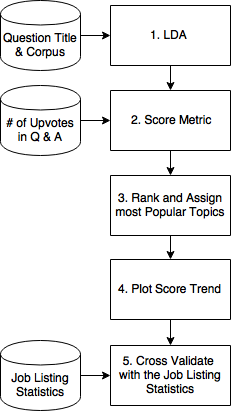
\includegraphics[width=5cm]{flowChart}
    \caption{General flowchart of the proposed algorithm}
    \label{fig:flowChart}
\end{figure}


\subsection{Data collection}
To analyze the score trend of the selected topics. We download the Q\&A entries from Stack Overflow and US technology job listing dataset from Kaggle.com. The file was separated by year, starting from 2008 to 2014. The title and corpus of the question entries were used for topic categorization with LDA. The upvotes of questions and upvotes of answers were extracted to calculate the score.

\subsection{Algorithm design}
The flowchart of the algorithm is shown in figure \ref{fig:flowChart}. The first step of the approach is to apply LDA algorithm to the titles and corpus of question entries. The granularity constant K will be tuned to lower the variance of the topic numbers in each category.
With the generated unnamed categories, the second step incorporated the votes of the questions and answers to calculate scores for each category.
In the third step, the categories with the top scores of all times from 2008 to 2014 were named according to the LDA most frequent keywords. Only the top scored topics were plotted in the trend comparison.
The score trend for the top ranked topics were plotted from 2008 to 2014. In our hypotheses, the score of the topics should match to the future popularities of the corresponding jobs.


%\subsection{Language and tool used}
We will mainly use python in this course project. Multiple open source packages would be used, including but not limited to pandas, NLTK, stop\_words, and genism. We will use the online tutorial "Latent Dirichlet Allocation (LDA) with Python" \cite{T1_Paper} as a reference to apply the LDA algorithm. 



%\subsubsection{a prototype (optional if time permit)}

\subsection{Scoring metric}

The scoring of the topics was calculated based on the supply and demand of the skills. High score indicates that the topic is popular with limited skill support. The score metric formula was designed as:

\begin{equation} \label{eq:1}
	Score = \frac{Demand - Supply}{n}
\end{equation}

$Demand$ is the number of upvotes in questions, $Supply$ is the number of upvotes in Answers, and $n$ is the number of entries, which normalizes the score for that specific topic. 

The voting system in Stack Overflow subtracted the downvotes from the upvotes. The cancellation effect automatically takes the downvotes into account. The formula is based on the assumption that the number of question upvotes could fully represent the demand while the number of answer upvotes represent the supply of talent in that specific topic.


\subsection{Testing against hypothesis}
To test against the hypothesis, we will check if the rank of the topic will predict the future popularity of  job fields by comparing the shape of the score curves with the job listing trends. Currently we have not decided on the source of the job listing statistics because the job titles have to fit in the categories summarized by the keywords generated from the LDA analysis. We will start searching the data when we obtain the results of the most popular topics from the LDA.


%\subsection{how to proof correctness (required by dissertation only)}
\section{Implementation}


\subsection{code (refer programming requirements)}
\subsection{design document and flowchart}
\section{Data Analysis and Discussion}

\subsection{output generation}

In order to finding the topics with least support, we need to calculate the support score for each topic, and for each year. To do so, first we will define the supportness score, and how we compute the score for each question; then we will sum the score of each questions which belong to a topic and year; then we compare the scores by topic, and by year.

The score of supportness for each question is represented by a supporting level score, which is calculated by the equation below:

\begin{gather*}
Score = \frac{(V_{q} - V{a})}{N}\\
\end{gather*}

In which $Score$ is the support level score for each topic at each year
\begin{gather*}
V_{q} = Number_{questionsUpvotes} - Number_{questionDownvotes}\\
V_{a} = Number_{answersUpvotes} - Number_{answersDownvotes} \\
N = Number_{questions}\\
\end{gather*}
After we train the LDA model, we input a document to the trained model, the result is as in the following format:\\

$LDAmodel (document 1) = \{p_{1}, p_{2}, p_{3}, p_{4}…..p_{k}\}$\\


where $p_{k}$ means the percentage of that document being categorized into topic $k$. We then multiply the $(V_{q} - V_{a})$ by $p_{k}$ and add the $1\times k$ array to the row of year in which the document belongs to.

In the end we will come up with a year versus topic matrix shown in Table \ref{table:tb1}.

\begin{table} 
	\centering
	\caption{Scoring matrix for each topics in each year}		
	\label{table:tb1}
	
	\begin{tabular}{ l l l l l }	
		\\		\hline
		Year & Topic 1 & Topic 2 & ... & Topic k\\ \hline  
		2008 & $Score_{T_1in2008}$ & $Score_{T_2in2008}$ &&$Score_{T_kin2008}$ \\
		2009 & $Score_{T_1in2009}$ & $Score_{T_2in2009}$ &&$Score_{T_kin2009}$ \\
		... &...&...&...&...		\\
		2016 & $Score_{T_1in2016}$ & $Score_{T_2in2016}$ &&$Score_{T_kin2016}$ \\
	\end{tabular}
\end{table}


With the scoring matrix, we calibrate each row of entry by dividing the entry with the sum of the row. Lastly we sum column to get the support for the topic that the column represents.


\subsection{output analysis}
\subsubsection{Support score for topics for year 2008-2016}


\begin{figure}
	\center
	\includegraphics[width=8cm]{100_1_Score.png}
	\caption{General flowchart of the proposed algorithm}
	\label{fig:waterfall}
\end{figure}


Figure \ref{fig:waterfall} showed how support level for each topic changes through the years. 

The equation of supportness score indicates that the lower the score, the more support the topic has.

From the diagram we found that the score for each topic is always negative, meaning that the $V_{a}$ is always larger than $V_{q}$. This indicates that for each year, the topics are always well supported in the community. Moreover, we found that the scores tends to be lower for previous years. This finding matches our intuition since the earlier the questions are posted, the more possible that the topic has been discussed.

\subsubsection{Compare results of different passes of same number of topics}
Further, we want to find the least score of the topics.

We tried different topic numbers (K) and passes (P) and trained multiple LDA models.
Figure \ref{fig:20_3} shows the score result for 20 topics and 3 passes. From the figure above we can see that topics 12 and 5 have the least support.


\begin{figure}
	\center
	\includegraphics[width=8cm]{20_3FindNoSupportTopics.png}
	\caption{Showing the score result for 20 topics and 3 passes. Topics 12 and 5 have the least support.}
	\label{fig:20_3}
\end{figure}

\begin{figure}
	\center
	\includegraphics[width=8cm]{50_3FindNoSupportTopics.png}
	\caption{Showing the score result for 50 topics and 3 passes. Topics 28 and 24 have the least support}
	\label{fig:50_3}
\end{figure}
\begin{figure}
	\center
	\includegraphics[width=8cm]{100_1FindNoSupportTopics.png}
	\caption{Showing the score result for 100 topics and 1 passes.Topics 14 and 33 have the least supported.}
	\label{fig:100_1}
\end{figure}

If we compare different k value by examining the top 10 keywords for each topic, we can summarize the result in Table \ref{T:kw}.





As we can see, the keywords are very different and hard to understand. Additionally, there is almost no similarity between the 2 topics with the lowest score for K = 20, 50, and 100. However, we did see similarity with “buffer2” appearing in both K=20 and K=50. We believe this shows that LDA is working, but still far from convergence. 


\subsubsection{Compare results of different passes of same number of topics}
Further, we compare the results obtained from different number of passes (p) on the same topic numbers (k).

For $k=20$, we generate the model on $p = 1$ and $p = 3$. The table \ref{T:kw2} shows the top keywords generated for each set. We can see that the keywords generated in 3 passes are generally more meaningful and more related to each other than the ones in just 1 pass. This proved that more passes in the LDA algorithm improve the cohesion of topics.


\begin{table}[ph]
	\center
	\caption{Top keywords for topic 12 when K = 20 for each pass}		
	%		\begin{tabularx}{c|c|c|c|c|c}
	\begin{tabular}{c|c}
		\hline
		Pass 1 & Pass 3\\
		\hline
		\begin{tabular}{@{}c@{}}
			jscrollpan\\
			newwordlist\\
			arg\\
			ios7\\
			scaley\\
			getus\\
			websecuritytest\\
			dataservic\\
			scalex\\
			use\_separ\\
		\end{tabular} &
		\begin{tabular}{@{}c@{}}
			uiview\\
			handlemarkclean\\
			nsjsonseri\\
			nsexcept\\
			dynload\\
			buffer2\\
			nilliteralconvert\\
			groups\_taglin\\
			282px\\
			mygoal\\
		\end{tabular}			
		
	\end{tabular}
	
	\label{T:kw2}

\end{table}

Similarly, we can evaluate topic 28 if k=50 as shown in Table \ref{T:kw3}


\begin{table}[ph]
	\center
	\caption{Top keywords for topic 28 when K = 50 for each pass}		
	%		\begin{tabularx}{c|c|c|c|c|c}
	\begin{tabular}{c|c|c}
		\hline
		Pass 1 & Pass 2 & Pass 3\\
		\hline
		\begin{tabular}{@{}c@{}}
			1020608401\\
			progrmmat\\
			385\\
			gdriveact\\
			properties\_home\_usage\_condit\\
			output\_file\_nam\\
			keep\_rat\\
			init\_data\\
			textfield\\
			u05d5\\
		\end{tabular} &
		\begin{tabular}{@{}c@{}}
			isexpand\\
			startdat\\
			setremembertoken\\
			910\\
			remindableinterfac\\
			telicat1ev\\
			pluss\\
			getstudentid\\
			nscalendar\\
			lead\_x	\\
		\end{tabular} &			
		\begin{tabular}{@{}c@{}}				
			cpe\\
			element\_nod\\
			buffer2\\
			gettextcont\\
			watchpoint\\
			setremembertoken\\
			begintransact\\
			getsystemservic\\
			90dp\\
			yocto\\
		\end{tabular}					
	\end{tabular}
	
	\label{T:kw3}
	
\end{table}
We can similarly see that topics are more coherent as the number of passes increases. Additionally, since a topic’s keywords change so much each pass, our model is far from converging. Thus, we can’t trust any of the results we have right now, since they are very likely to change significantly if we were to run one more iteration of LDA. 



\subsection{compare output against hypothesis}
We hypothesized that we can identify which topics have limited support on Stack Overflow based on our scoring metrics. Our graph of score vs. topic vs. year shows that our scoring metric works because older questions that have more time to receive answers have a better score (more negative score means more support). The topics identified as having the least support are not stable, and changed significantly between passes of LDA as well as when we changed K, the number of topics. Thus, our data does not support a solid conclusion in identifying which topics have the least support on Stack Overflow.

\subsection{abnormal case explanation (the most important task)}
There are a lot of abnormal cases involving the top words in each topic. One example from running LDA with 100 topics was “intoxicatedbia”, a word that shows up only once on Stack Overflow and hardly anywhere else in the whole internet. It is troubling that such a rare word would be characterized as one of the top words in a topic. We believe that this is likely due to the fact that we removed so many stop words as well as only running 1 pass (iteration) of the LDA algorithm, so this model was likely inaccurate.
Another set of abnormal top “words” were just numbers. We found that numbers showed up quite often in the list of top words of a topic when we did a low number of passes. Those numbers were almost always meaningless, and ended up being noise that made the analysis of each topic more difficult. 
Another abnormal case stemmed from our stemming function. We used a stemming function that truncated words down to their roots (e.g. talking, talker, and talkative were all truncated down to talk). While this can improve accuracy by linking similar words together, we noticed that our stemming function may have trimmed too much from the ends of some words. One common word that we found was “iphon”, which obviously related to iphones. However, the root word would be iphone, not iphon. Another example is “forl”, which we believe is the root of “for loop”. These are just representative examples of how our stemming function may have gone too far in truncating off the ends of words and eliminated whitespace between words. One consequence of this is that understanding what actual words are in each topic is quite difficult.

\subsection{discussion}
Our research and analysis has taught us many things. We learned the value of parsing data well, since a large portion of our work was dedicated to collecting, cleaning, and parsing the data into a format suitable for the LDA model to train on. We also ran into limitations regarding computing resources. We had a lot of text data to train our LDA model on, so it took many hours to train our model. We even ran into memory issues from not enough RAM on our computer to hold all of the data at once. This taught us some of the complexities of working with big data, since I/O delays from moving data between RAM and disk are far higher than CPU computing times. Due to our computing restraints, our LDA model was not as accurate as we had hoped it to be, and this limited our results to some degree.




%\subsection{compare output against hypothesis}
%\subsection{abnormal case explanation (the most important task)}
%\subsection{statistic regression}
%\subsection{discussion}
\section{Conclusions and Recommendations}


\subsection{summary and conclusions}
Our results from LDA were very unstable, changing significantly between each pass and as we changed the number of topics. Since we couldn’t find consistency in the topics, we can’t say with confidence that the topics that have the least support based on our scoring metrics are actually the topics with the least support. Thus, we can’t identify topics with limited support on Stack Overflow. However, we have found that our scoring metrics do work because older questions have more support as people have had more time to respond. This shows that we are working in the right direction, but need more time to develop the LDA model so that we can find a consistent set of topics.
\subsection{recommendations for future studies}
Future research can get better results by running our LDA models for a longer period of time (i.e. more passes to fit LDA). We were limited to 3 passes because of time constraints for fitting the model, but more passes would increase the accuracy. In addition, because fitting the LDA model took so long, further research can be done to explore different numbers of topics to fit LDA to and how that affects the results. We analyzed 20, 50, and 100 topics, but more or fewer topics may show insights that we have not seen before. Another area worth exploring would be how the number of stop words removes affects LDA accuracy. We removed a large amount of stop words, approximately 500,000, and this may have been too many. It is possible that removing fewer stop words would result in a more accurate model. One thing we did find is that numbers showed up quite frequently as top words in a topic, even though they often carry no specific meaning. In the future, we recommend adding numbers to the list of stopwords.

Another avenue of analysis would be to explore different scoring metrics to measure topic support. We noticed that for every topic, there were more answer upvotes than question upvotes, so our scoring metric was always negative. This is not bad in and of itself, but this may be an indicator that a different scoring metric may be better in evaluating support for a topic.

A major area of analysis that we were not able to touch was to correlate which topics have limited support with the job postings data for each year. The hypothesis is that topics with limited support will have more open jobs that year because there is a lack of talent in that topic. We could not find suitable job postings data that was categorized by year, so we weren’t able to perform this analysis. However, this is a very important area of research because if the hypothesis is true, then we can predict how many jobs in certain fields will remain open based on the related Stack Overflow questions and answers.



\begin{thebibliography}{1}



\bibitem{N1_Paper}
Christoffer Rosen and Emad Shihab, \emph{What are mobile developers asking about? A large scale study using stack overflow}. \hskip 1em plus 0.5em minus 0.4em\relax Empirical Software Engineering, 2016

\bibitem{N2_Paper}
R.K. Ranjitha and Sanjay Singh, \emph{Is Stack Overflow Overflowing With Questions and Tags}. \hskip 1em plus 0.5em minus 0.4em\relax ACM Digital Library, 2015


\bibitem{N3_Paper}
Fabio Calefato, Filippo Lanubile, and Nicole Novielli, \emph{Moving to Stack Overflow: Best-Answer Prediction in Legacy Developer Forums}. \hskip 1em plus 0.5em minus 0.4em\relax ACM Digital Library, 2016

\bibitem{T1_Paper}
Jordan Barber (2017, Nov. 6), \emph{Latent Dirichlet Allocation (LDA) with Python}. \hskip 1em plus 0.5em minus 0.4em\relax Retrived from \url{https://rstudio-pubs-static.s3.amazonaws.com/79360_850b2a69980c4488b1db95987a24867a.html}



\end{thebibliography}


%\newpage 
\onecolumn
%
\section*{Appendices}
\addcontentsline{toc}{section}{Appendices}

\begin{table*}[ph]
	
	\caption{$N_{t} =$ ID of the Topic. Table shows top 10 keywords}		
	%		\begin{tabularx}{c|c|c|c|c|c}
	\begin{tabularx}{\textwidth}{@{}l*{10}{C}c@{}}
		
		\hline
		\multicolumn{2}{c}{$k = 20, P = 3$} & \multicolumn{2}{c}{$k = 50, P = 3$}  & \multicolumn{2}{c}{$k = 100, P = 1$} \\
		\hline
		$N_{t}$ & Keywords & $N_{t}$ & Keywords & $N_{t}$ & Keywords \\
		\hline
		12 & 
		\begin{tabular}{@{}c@{}}
			uiview \\
			handlemarkclean\\
			nsjsonseri      	\\
			nsexcept         	\\
			dynload          	\\
			buffer2\\
			nilliteralconvert\\
			groups\_taglin	\\
			282px\\
			mygoal\\
			
		\end{tabular}				
		& 28 & 
		\begin{tabular}{@{}c@{}}
			cpe\\
			element\_nod\\
			buffer2\\
			gettextcont\\
			watchpoint\\
			setremembertoken\\
			begintransact\\
			getsystemservic\\
			90dp\\
			yocto\\
		\end{tabular}			
		&14 &
		
		\begin{tabular}{@{}c@{}}
			openerp	\\
			netsvc	\\
			View\_op\_timetable\_postpon\\
			postponed\_op\_time\\
			tpastebi\\
			openeducat	\\
			tx	\\
			cache\_t	\\
			headeralign	\\
			col6\\
		\end{tabular}\\
		\hline
		5 & 
		\begin{tabular}{@{}c@{}}
			93342519      	\\
			sysutil\\
			tform	\\
			libjvm\\
			0x0000000000000000           	\\
			1190 	\\
			responsetext\\
			8f\\
			myobj  \\
			Clientwidth\\
			
			
		\end{tabular}				
		& 24 & 
		\begin{tabular}{@{}c@{}}
			jscrollpan\\
			usedd\\
			allengag\\
			setvis\\
			jqueryui\\
			aarray\\
			ijsonancestor\\
			113l\\
			jdialog\\
			menupanel\\
			
		\end{tabular}			
		&33 &
		
		\begin{tabular}{@{}c@{}}
			efilesubmisiond\\
			x100	\\
			dspaceservlet	\\
			filepath	\\
			image1\\
			acct	\\
			net\_sal	\\
			organizationid\\
			simplxml	\\
			allengageform\\
			
		\end{tabular}\\
		
		\hline
	\end{tabularx}
	
	\label{T:kw}
	
\end{table*}

\begin{figure}[ht]
	\centering
	\includegraphics[width=15cm]{FlowD.png}
	\caption{Program flowchart}
	
	\label{fig:program_flowchart}
\end{figure}
%\begin{sidewaysfigure}[ht]
%	\includegraphics[width=20cm]{FlowD.png}
%\caption{Program flowchart}
%\label{fig:program_flowchart}
%\end{sidewaysfigure}



\end{document}


